%! Author = wolfram_e_laube
%! Date = 06.05.24

\item[(a)]
The spectrum is plotted using Python as follows:

\begin{verbatim}
import numpy as np
import matplotlib.pyplot as plt

# Parameters
fs_analog = 100e3  # 100 kHz
f1 = 4e3  # 4 kHz
f2 = 6e3  # 6 kHz
t_end = 2e-3  # 2 ms

# Time vector
t = np.arange(0, t_end, 1/fs_analog)

# Analog signal
x_t = np.sin(2 * np.pi * f1 * t) + np.sin(2 * np.pi * f2 * t)

# FFT to compute the spectrum
n = len(t)
freqs = np.fft.fftfreq(n, d=1/fs_analog)
spectrum = np.fft.fft(x_t)

# Plotting
plt.figure()
plt.plot(freqs[:n // 2] / 1e3, np.abs(spectrum[:n // 2]))
plt.xlabel('Frequency (kHz)')
plt.ylabel('Amplitude')
plt.title('Spectrum of x(t)')
plt.grid(True)
plt.show()
\end{verbatim}

\begin{figure}[h]
    \centering
    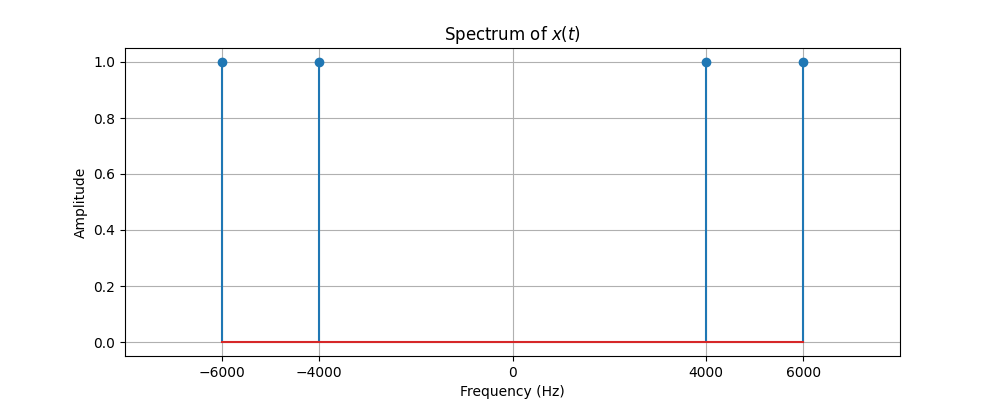
\includegraphics[width=0.49\textwidth]{fig/ex1_a_plot}
    \caption{Spectrum of \(x(t)\)}
    \label{fig:ex1_a_plot}
\end{figure}
